\documentclass[12pt]{notes}\usepackage[]{graphicx}\usepackage[]{color}
% maxwidth is the original width if it is less than linewidth
% otherwise use linewidth (to make sure the graphics do not exceed the margin)
\makeatletter
\def\maxwidth{ %
  \ifdim\Gin@nat@width>\linewidth
    \linewidth
  \else
    \Gin@nat@width
  \fi
}
\makeatother

\definecolor{fgcolor}{rgb}{0.345, 0.345, 0.345}
\newcommand{\hlnum}[1]{\textcolor[rgb]{0.686,0.059,0.569}{#1}}%
\newcommand{\hlstr}[1]{\textcolor[rgb]{0.192,0.494,0.8}{#1}}%
\newcommand{\hlcom}[1]{\textcolor[rgb]{0.678,0.584,0.686}{\textit{#1}}}%
\newcommand{\hlopt}[1]{\textcolor[rgb]{0,0,0}{#1}}%
\newcommand{\hlstd}[1]{\textcolor[rgb]{0.345,0.345,0.345}{#1}}%
\newcommand{\hlkwa}[1]{\textcolor[rgb]{0.161,0.373,0.58}{\textbf{#1}}}%
\newcommand{\hlkwb}[1]{\textcolor[rgb]{0.69,0.353,0.396}{#1}}%
\newcommand{\hlkwc}[1]{\textcolor[rgb]{0.333,0.667,0.333}{#1}}%
\newcommand{\hlkwd}[1]{\textcolor[rgb]{0.737,0.353,0.396}{\textbf{#1}}}%
\let\hlipl\hlkwb

\usepackage{framed}
\makeatletter
\newenvironment{kframe}{%
 \def\at@end@of@kframe{}%
 \ifinner\ifhmode%
  \def\at@end@of@kframe{\end{minipage}}%
  \begin{minipage}{\columnwidth}%
 \fi\fi%
 \def\FrameCommand##1{\hskip\@totalleftmargin \hskip-\fboxsep
 \colorbox{shadecolor}{##1}\hskip-\fboxsep
     % There is no \\@totalrightmargin, so:
     \hskip-\linewidth \hskip-\@totalleftmargin \hskip\columnwidth}%
 \MakeFramed {\advance\hsize-\width
   \@totalleftmargin\z@ \linewidth\hsize
   \@setminipage}}%
 {\par\unskip\endMakeFramed%
 \at@end@of@kframe}
\makeatother

\definecolor{shadecolor}{rgb}{.97, .97, .97}
\definecolor{messagecolor}{rgb}{0, 0, 0}
\definecolor{warningcolor}{rgb}{1, 0, 1}
\definecolor{errorcolor}{rgb}{1, 0, 0}
\newenvironment{knitrout}{}{} % an empty environment to be redefined in TeX

\usepackage{alltt}

% Command for Questions
%\question{}

% Command for Notes
% \note{}

% Code to create a minipage where you can type in class notes.
%%\begin{minipage}[l][2cm][c]{\textwidth}
%\begin{comment}

%\end{comment}
%%\end{minipage}

% In order for the minted code to run, we had to create a new compilation routine called pdflatex+shellEscape.
% This includes a --shell-escape command which should ONLY be used when pygmentized is required as it compromises security.
% We also had to add pygmentize (a python package) to the system path (BEFORE miktex) and then restart the computer.
\usepackage{listings}
\usepackage{minted}
\usemintedstyle{borland}
\lstset{language=SAS,
  breaklines=true,
  basicstyle=\ttfamily\bfseries,
  columns=fixed,
  keepspaces=true,
  identifierstyle=\color{blue}\ttfamily,
  keywordstyle=\color{cyan}\ttfamily,
  stringstyle=\color{purple}\ttfamily,
  commentstyle=\color{green}\ttfamily,
  }



% Begin Document
%==============================================================================
\IfFileExists{upquote.sty}{\usepackage{upquote}}{}
\begin{document}
%\SweaveOpts{concordance=TRUE}
% Include the Title of the Handout
\ntitle{1.4: Data Exploration}

% Include Numbered Sections
\section{Why Data Exploration}

Data Modeling is a lot like:

\begin{figure}[H]
\centering
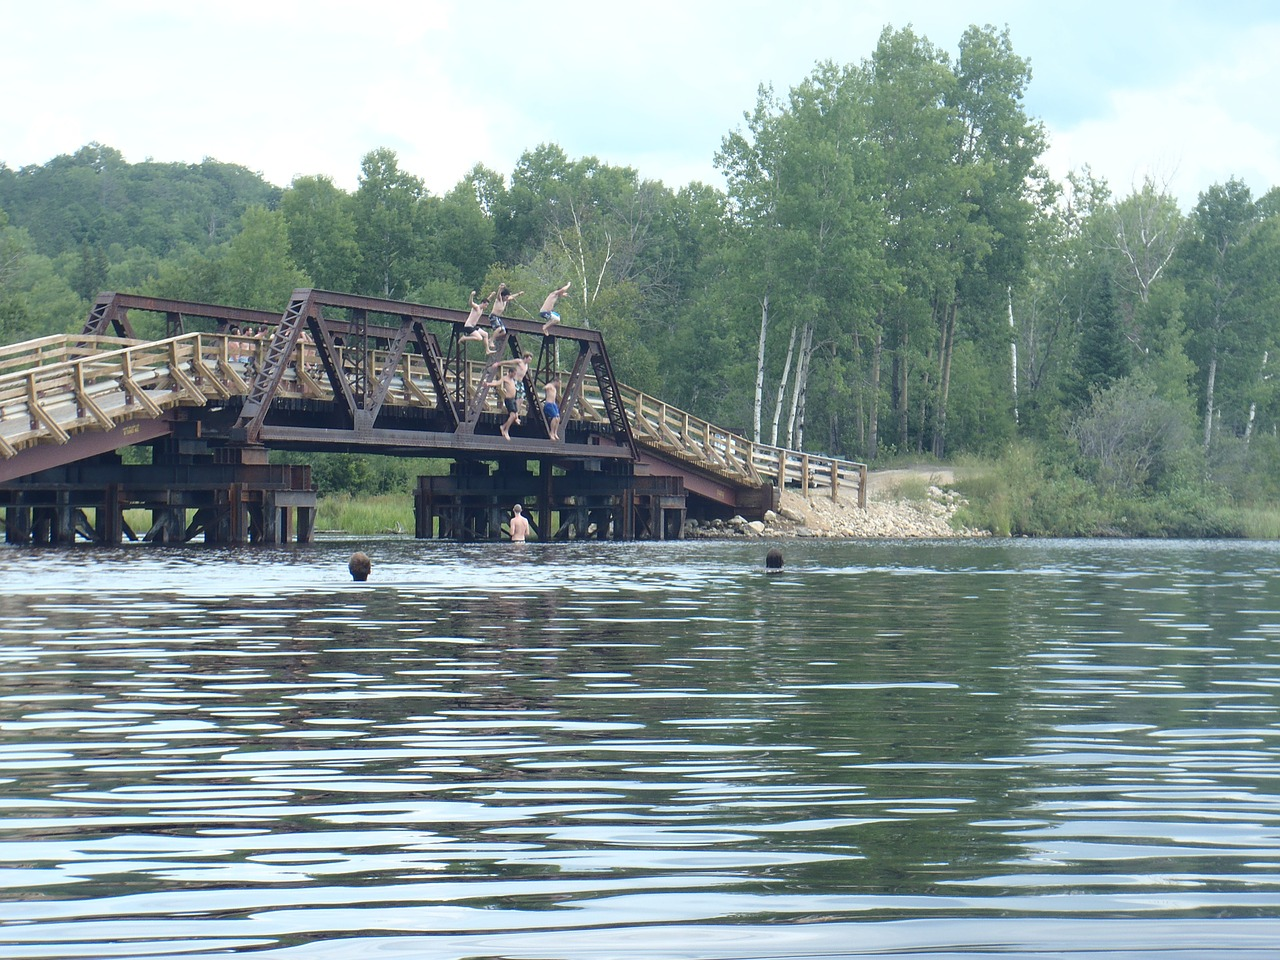
\includegraphics[width=0.5\textwidth]{../figures/module1/bridgeJumping.jpg}
\end{figure}

In order to avoid disaster, you need to \textbf{look} before you \textbf{jump}.

\nspace
Example:
Consider four scenarios where we use to create a model that uses values of $x$ to predict values of $y$. We make the assumption in each case that the data can be modeled as
\begin{equation}
Y_i = \beta_0 + \beta_1X_{i,1} + \epsilon_i
\end{equation}

This assumption means that we assume that $X$ and $Y$ share a linear relationship. That is, as $X$ increases, $Y$ will increase proportionally. We will explore this further in Handout 2.1.

\nspace
Data Explorations BEFORE modeling will help us to detect:
\begin{itemize}
\item Skewed distributions
\item Outlier points
\item Non-linear trends
\end{itemize}

Often, we can use \textbf{variable transformations} to get data that are normal, or at least symmetric, in distribution.

\begin{minipage}[l][3cm][c]{\textwidth}
%\begin{comment}
\note{Why symmetric data? Consider the ``door hinge'' problem.}
%\end{comment}
\end{minipage}

\textbf{Common Exploratory Plots}
\begin{itemize}
\item \textbf{Boxplots:}: Show the five quartlies of the data (min, 25th percentile, median, 75th percentile, and maximum).
\begin{itemize}
\item Values that are farther than 1.5*IQR (Interquartile Range, which is the 75th percentile minus the 25 percentile) above the 75th percentile or below the 25th percentile are typically plotted as ``outlier'' points.
\item Great way to quickly summarize the range of values.

\begin{knitrout}
\definecolor{shadecolor}{rgb}{0.969, 0.969, 0.969}\color{fgcolor}\begin{kframe}
\begin{alltt}
\hlkwd{library}\hlstd{(stat5100)}
\hlkwd{data}\hlstd{(college)}

\hlkwd{boxplot}\hlstd{(college}\hlopt{$}\hlstd{gpa,} \hlkwc{main} \hlstd{=} \hlstr{"Sample Boxplot of GPA"}\hlstd{,} \hlkwc{ylab} \hlstd{=} \hlstr{"GPA"}\hlstd{)}
\end{alltt}
\end{kframe}

{\centering 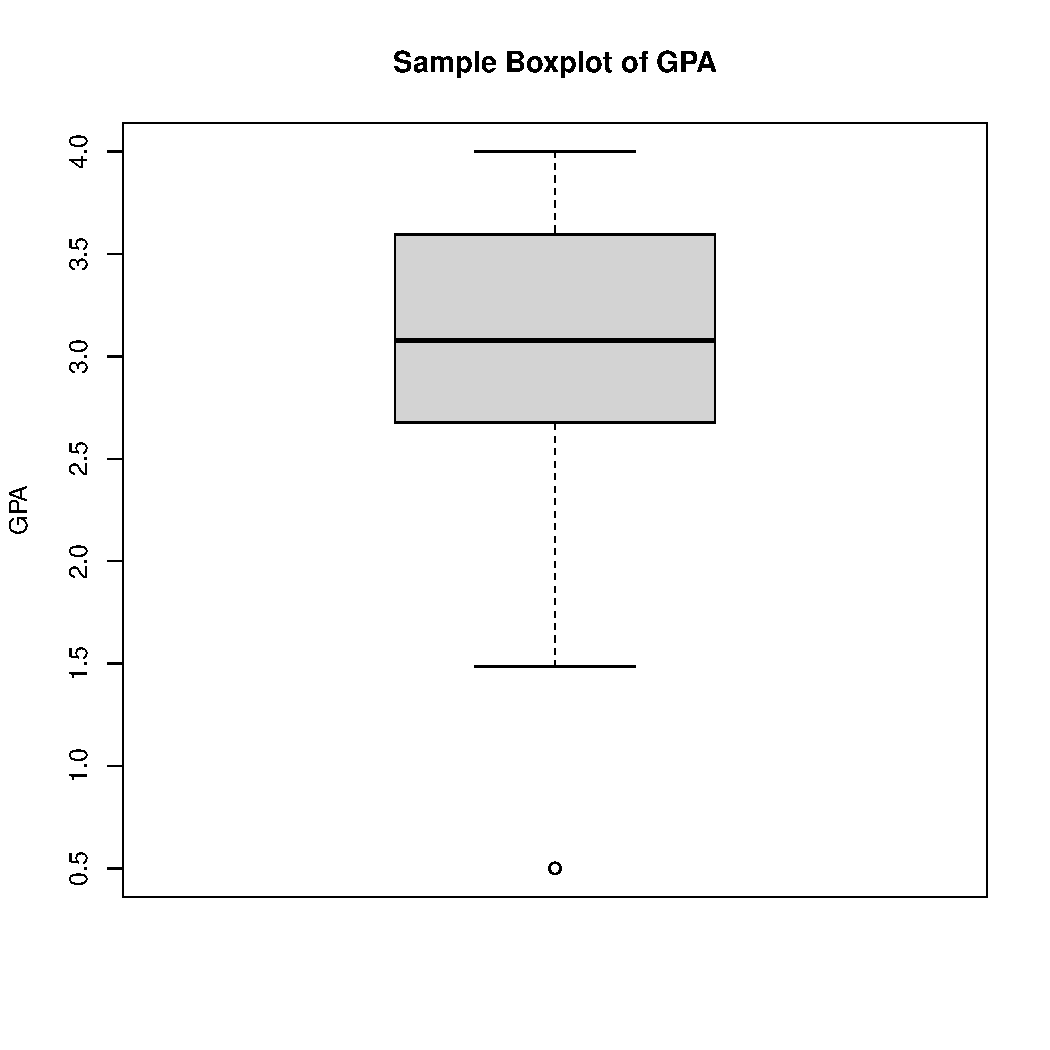
\includegraphics[width=0.6\textwidth]{figure/unnamed-chunk-1-1} 

}



\end{knitrout}

\end{itemize}
\item \textbf{Histograms:} Use bins to show the number of observations in a range.
\begin{itemize}
\item Help us to visualize the distribution of the data by imagining a smooth curve running along the top of the bins.
\item Word of caution: the choice of bin width can drastically change the shape of a histogram.
\end{itemize}

\begin{knitrout}
\definecolor{shadecolor}{rgb}{0.969, 0.969, 0.969}\color{fgcolor}\begin{kframe}
\begin{alltt}
\hlkwd{hist}\hlstd{(college}\hlopt{$}\hlstd{gpa,} \hlkwc{main} \hlstd{=} \hlstr{"Sample Histogram of GPA"}\hlstd{,} \hlkwc{xlab} \hlstd{=} \hlstr{"GPA"}\hlstd{)}
\end{alltt}
\end{kframe}

{\centering 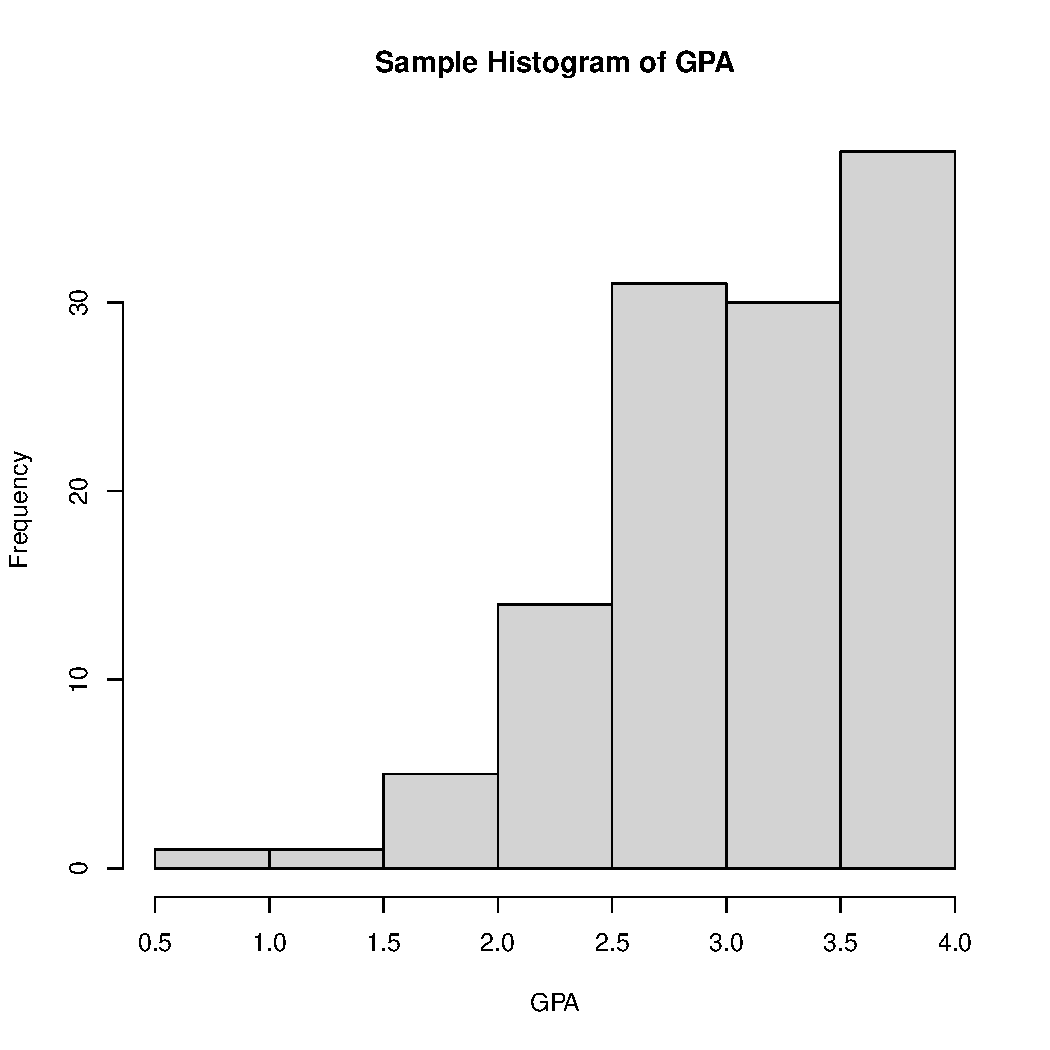
\includegraphics[width=0.6\textwidth]{figure/unnamed-chunk-2-1} 

}



\end{knitrout}


\item \textbf{QQ Plot:} ``Quantile Comparison'' plots help to easily compare the observed distribution of points to a theoretical (typically normal) distribution.
\begin{itemize}
\item Plots the data quantiles against the theoretical quantiles of similar observations that are normal in distribution.
\item Points that closely follow the diagonal line indicate that the observed data follow the theoretical distribution.
\item While they don't help to visualize shape, qqplots are superior to histograms as a visual check for normality.
\end{itemize}

\begin{knitrout}
\definecolor{shadecolor}{rgb}{0.969, 0.969, 0.969}\color{fgcolor}\begin{kframe}
\begin{alltt}
\hlkwd{qqnorm}\hlstd{(college}\hlopt{$}\hlstd{gpa,} \hlkwc{main} \hlstd{=} \hlstr{"Sample Q-Q Plot"}\hlstd{)}
\hlkwd{qqline}\hlstd{(college}\hlopt{$}\hlstd{gpa)}
\end{alltt}
\end{kframe}

{\centering 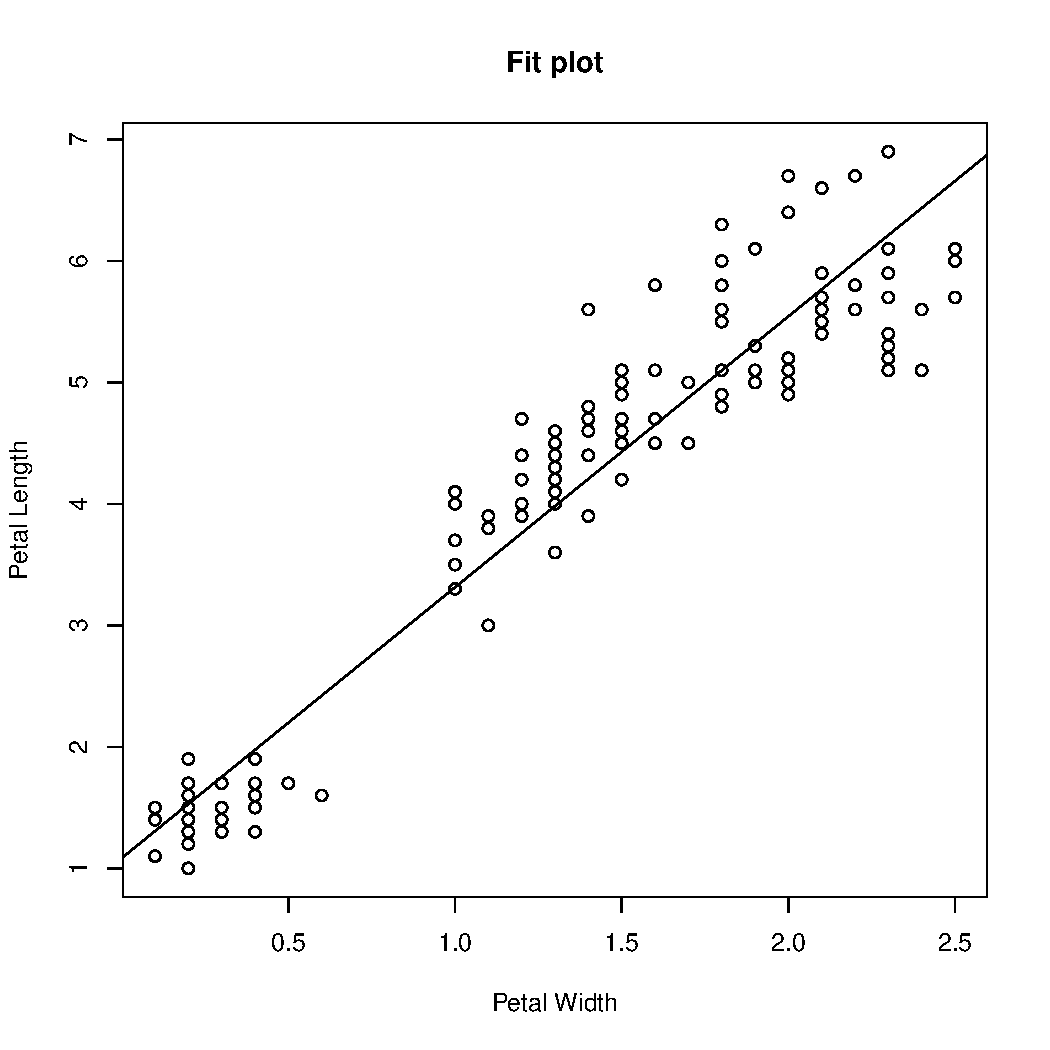
\includegraphics[width=0.6\textwidth]{figure/unnamed-chunk-3-1} 

}



\end{knitrout}

\textit{(The above shows that GPA is clearly not normally distributed. If they were, then the data points would lie on the line very nicely.)}

\item \textbf{Scatterplots:} Plots paired observations from two variables as points on a two-dimensional plot.
\begin{itemize}
\item Excellent way to determine if two variables share a relationship.
\item Can combine in a \textbf{scatterplot matrix} when looking at relationships between more than two variables.
\item Subject to \textbf{overplotting} when you have thousands of observations that you are trying to plot at the same time.
\end{itemize}

\begin{knitrout}
\definecolor{shadecolor}{rgb}{0.969, 0.969, 0.969}\color{fgcolor}\begin{kframe}
\begin{alltt}
\hlkwd{plot}\hlstd{(college}\hlopt{$}\hlstd{act, college}\hlopt{$}\hlstd{gpa,} \hlkwc{main} \hlstd{=} \hlstr{"Sample Scatterplot of GPA vs ACT"}\hlstd{,}
     \hlkwc{xlab} \hlstd{=} \hlstr{"ACT Score"}\hlstd{,} \hlkwc{ylab} \hlstd{=} \hlstr{"GPA"}\hlstd{)}
\end{alltt}
\end{kframe}

{\centering 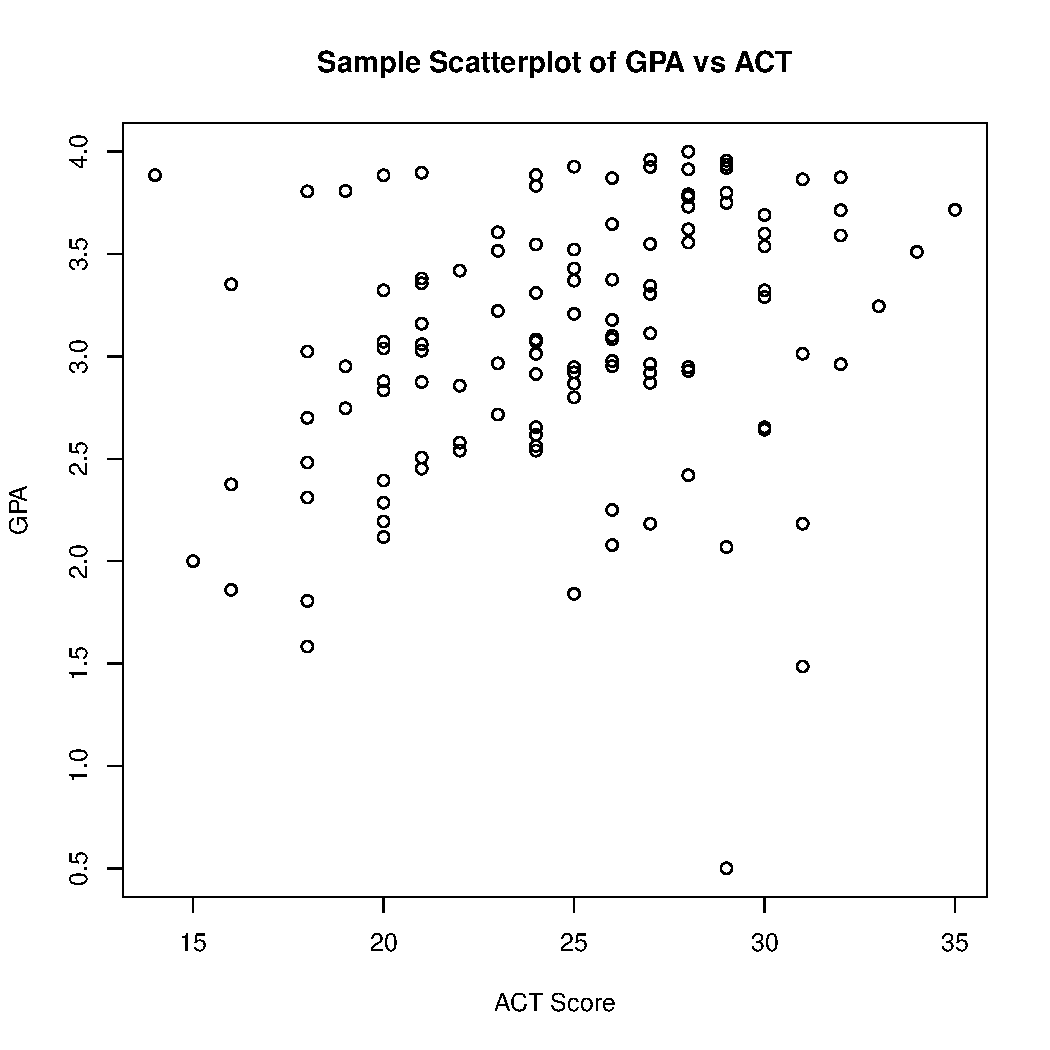
\includegraphics[width=0.6\textwidth]{figure/unnamed-chunk-4-1} 

}



\end{knitrout}


\end{itemize} % End the list of graphics.

\nspace
See \textbf{Handout 1.4.2} for an extended example in R of data explorations.

















% End the Document
%==============================================================================
\end{document}
